\documentclass{beamer}

% Required packages
\usepackage{tikz}
\usepackage{amsmath}
\usepackage{listings}
\usepackage{xcolor}

% Define custom colors
\definecolor{ds9blue}{RGB}{25,25,112}
\definecolor{ds9gold}{RGB}{218,165,32}
\definecolor{ds9grey}{RGB}{105,105,105}
\definecolor{ds9red}{RGB}{178,34,34}

% Theme configuration
\usetheme{Madrid}
\usecolortheme{whale}
\setbeamercolor{structure}{fg=ds9blue}
\setbeamercolor{alerted text}{fg=ds9red}
\setbeamercolor{example text}{fg=ds9gold}

% Title page configuration
\title[Big O Notation]{CS12: Introduction to Big O Notation}
\subtitle{Understanding Algorithm Efficiency}
\author[Mr. Gullo]{Mr. Gullo}
\date{}


\begin{document}

% Title page
\begin{frame}
    \titlepage
\end{frame}

% Table of Contents
\begin{frame}{Overview}
    \tableofcontents
\end{frame}

% Learning objectives
\begin{frame}{Learning Objectives}
    By the end of this lesson, you will be able to:
    \begin{itemize}
        \item Define algorithm efficiency in your own words
        \item Identify and explain common Big O notations
        \item Analyze simple algorithms to determine their time complexity
        \item Compare different algorithms based on their efficiency
    \end{itemize}
\end{frame}

% Introduction to Big O
\begin{frame}{What is Big O Notation?}
    \begin{block}{Definition}
        Big O notation measures how an algorithm's running time or space requirements grow as the input size increases.
    \end{block}
    
    \begin{itemize}
        \item Think of it as a way to measure an algorithm's speed
        \item Helps us compare different solutions
        \item Focuses on the worst-case scenario
        \item Ignores smaller details and focuses on the big picture
    \end{itemize}
\end{frame}

% Visual comparison
\begin{frame}{How Different Algorithms Grow}
    \begin{center}
    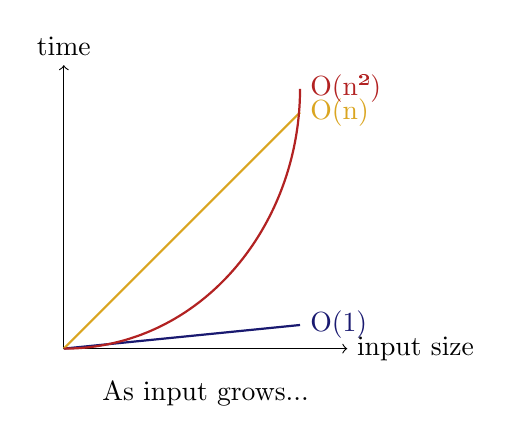
\begin{tikzpicture}[scale=0.6]
        \draw[->] (0,0) -- (6,0) node[right] {input size};
        \draw[->] (0,0) -- (0,6) node[above] {time};
        \draw[ds9blue, thick] (0,0) -- (5,0.5) node[right] {O(1)};
        \draw[ds9gold, thick] (0,0) -- (5,5) node[right] {O(n)};
        \draw[ds9red, thick] (0,0) to[out=0,in=270] (5,5.5) node[right] {O(n²)};
        
        \node[below] at (3,-0.5) {As input grows...};
    \end{tikzpicture}
    \end{center}
\end{frame}

% Real-world analogies
\begin{frame}{Understanding Through Real Examples}
    \begin{columns}
        \column{0.5\textwidth}
        \textbf{O(1) - Constant Time}
        \begin{itemize}
            \item Finding a book on your desk
            \item Looking up array element by index
        \end{itemize}
        
        \textbf{O(n) - Linear Time}
        \begin{itemize}
            \item Searching through a line of books
            \item Finding maximum in unsorted array
        \end{itemize}
        
        \column{0.5\textwidth}
        \textbf{O(n²) - Quadratic Time}
        \begin{itemize}
            \item Comparing every book with others
            \item Bubble sort algorithm
        \end{itemize}
        
        \textbf{O(log n) - Logarithmic Time}
        \begin{itemize}
            \item Finding word in dictionary
            \item Binary search
        \end{itemize}
    \end{columns}
\end{frame}

% I Do Example
\begin{frame}[fragile]{I Do: Analyzing Linear Search}
    \begin{block}{Problem}
        Let's analyze this linear search algorithm:
    \end{block}
    \begin{lstlisting}[language=C++, basicstyle=\small]
int linearSearch(int arr[], int n, int x) {
    for(int i = 0; i < n; i++) {
        if(arr[i] == x) {
            return i;  // Found it!
        }
    }
    return -1;  // Not found
}
    \end{lstlisting}
    \begin{itemize}
        \item Time Complexity: O(n)
        \item Why? In worst case, we check every element
    \end{itemize}
\end{frame}

% We Do Example
\begin{frame}[fragile]{We Do: Let's Analyze Together}
    \begin{block}{What's the time complexity?}
    \end{block}
    \begin{lstlisting}[language=C++, basicstyle=\small]
void printPairs(int arr[], int n) {
    for(int i = 0; i < n; i++) {
        for(int j = 0; j < n; j++) {
            cout << arr[i] << "," 
                 << arr[j] << endl;
        }
    }
}
    \end{lstlisting}
    \pause
    \begin{itemize}
        \item Let's count the operations...
        \item Outer loop runs n times
        \item For each outer loop, inner loop runs n times
        \item Total operations: n × n = n²
    \end{itemize}
\end{frame}

% You Do Example
\begin{frame}{You Do: Practice Time!}
    \begin{block}{Analyze These Operations}
        Determine the Big O notation for:
    \end{block}
    \begin{enumerate}
        \item Getting the first element of an array
        \item Finding the maximum value in an unsorted array
        \item Checking if a number is even or odd
    \end{enumerate}
    \pause
    \begin{alertblock}{Solutions}
        \begin{enumerate}
            \item O(1) - Direct access, no matter the size
            \item O(n) - Must check every element once
            \item O(1) - Single operation, size independent
        \end{enumerate}
    \end{alertblock}
\end{frame}

% Summary
\begin{frame}{Key Takeaways}
    \begin{block}{Remember These Points}
        \begin{itemize}
            \item Big O notation helps us measure efficiency
            \item Most common notations: O(1), O(n), O(n²)
            \item Consider how performance changes with input size
            \item Different problems require different solutions
        \end{itemize}
    \end{block}
    
    \begin{alertblock}{Practice Makes Perfect}
        Try analyzing algorithms you write in your own code!
    \end{alertblock}
\end{frame}

\end{document}